% Options for packages loaded elsewhere
\PassOptionsToPackage{unicode}{hyperref}
\PassOptionsToPackage{hyphens}{url}
%
\documentclass[
]{article}
\usepackage{lmodern}
\usepackage{amssymb,amsmath}
\usepackage{ifxetex,ifluatex}
\ifnum 0\ifxetex 1\fi\ifluatex 1\fi=0 % if pdftex
  \usepackage[T1]{fontenc}
  \usepackage[utf8]{inputenc}
  \usepackage{textcomp} % provide euro and other symbols
\else % if luatex or xetex
  \usepackage{unicode-math}
  \defaultfontfeatures{Scale=MatchLowercase}
  \defaultfontfeatures[\rmfamily]{Ligatures=TeX,Scale=1}
\fi
% Use upquote if available, for straight quotes in verbatim environments
\IfFileExists{upquote.sty}{\usepackage{upquote}}{}
\IfFileExists{microtype.sty}{% use microtype if available
  \usepackage[]{microtype}
  \UseMicrotypeSet[protrusion]{basicmath} % disable protrusion for tt fonts
}{}
\makeatletter
\@ifundefined{KOMAClassName}{% if non-KOMA class
  \IfFileExists{parskip.sty}{%
    \usepackage{parskip}
  }{% else
    \setlength{\parindent}{0pt}
    \setlength{\parskip}{6pt plus 2pt minus 1pt}}
}{% if KOMA class
  \KOMAoptions{parskip=half}}
\makeatother
\usepackage{xcolor}
\IfFileExists{xurl.sty}{\usepackage{xurl}}{} % add URL line breaks if available
\IfFileExists{bookmark.sty}{\usepackage{bookmark}}{\usepackage{hyperref}}
\hypersetup{
  pdfauthor={Michael Gaunt mike.gaunt@wsp.com},
  hidelinks,
  pdfcreator={LaTeX via pandoc}}
\urlstyle{same} % disable monospaced font for URLs
\usepackage[margin=1in]{geometry}
\usepackage{graphicx,grffile}
\makeatletter
\def\maxwidth{\ifdim\Gin@nat@width>\linewidth\linewidth\else\Gin@nat@width\fi}
\def\maxheight{\ifdim\Gin@nat@height>\textheight\textheight\else\Gin@nat@height\fi}
\makeatother
% Scale images if necessary, so that they will not overflow the page
% margins by default, and it is still possible to overwrite the defaults
% using explicit options in \includegraphics[width, height, ...]{}
\setkeys{Gin}{width=\maxwidth,height=\maxheight,keepaspectratio}
% Set default figure placement to htbp
\makeatletter
\def\fps@figure{htbp}
\makeatother
\setlength{\emergencystretch}{3em} % prevent overfull lines
\providecommand{\tightlist}{%
  \setlength{\itemsep}{0pt}\setlength{\parskip}{0pt}}
\setcounter{secnumdepth}{-\maxdimen} % remove section numbering

\title{
\includegraphics[width=9in,height=\textheight]{./www/flatart_long.jpg}}
\author{Michael Gaunt
\href{mailto:mike.gaunt@wsp.com}{\nolinkurl{mike.gaunt@wsp.com}}}
\date{2020-11-11}

\begin{document}
\maketitle

{
\setcounter{tocdepth}{2}
\tableofcontents
}
\hypertarget{overview}{%
\section{Overview}\label{overview}}

The Ultra High Speed Ground Transportation (UHSGT) Planning Dashboard is
a tool to investigate the Eugene, OR to Vancouver, British Columbia
corridor for the purposes of planning a potential UGSGT system in the
Pacific Northwest (PNW). This dashboard is a web-based application - it
requires no specific technical domain knowledge to use and gather
information from. This dashboard brings together a variety of data
streams which work together to represent the governance and
transportation networks which make up the corridor. Combining all of
this data in one place allows the user to inspect spatial connections
between different features and retrieve statistics with ease and
immediacy. In addition, this tool provides the ability for users to
define their own spatial geometries and investigate how those new
features interact with existing map layers, boundaries, and features.

\hypertarget{dashboard-features}{%
\subsection{Dashboard Features}\label{dashboard-features}}

The main features included in this map are as follows:

\begin{itemize}
\tightlist
\item
  A large interactive map of the corridor from Eugene, OR. to Vancouver,
  British Columbia

  \begin{itemize}
  \tightlist
  \item
    This map contains a number of different layers and displays layer
    feature meta-data
  \item
    This map encourages the user to explore the corridor at a high level
  \end{itemize}
\item
  The ability for users to provide/create their own geometry and see how
  it interacts with the default map

  \begin{itemize}
  \tightlist
  \item
    This feature increases the user's ability to target areas and map
    layers
  \item
    Users can download these features (.shp format)
  \end{itemize}
\end{itemize}

\hypertarget{user-manual}{%
\section{User Manual}\label{user-manual}}

This document stands to serve as an operation manual on how to use and
navigate the dashboard. In addition to this document, the dashboard also
contains a number of information buttons that can be clicked on that
provide information about a particular page or dashboard functionality.

\hypertarget{dashboard-navigation}{%
\subsection{Dashboard Navigation}\label{dashboard-navigation}}

The dashboard use-interface (UI) is composed of three sections - the top
header bar, the left sidebar, and the main display.

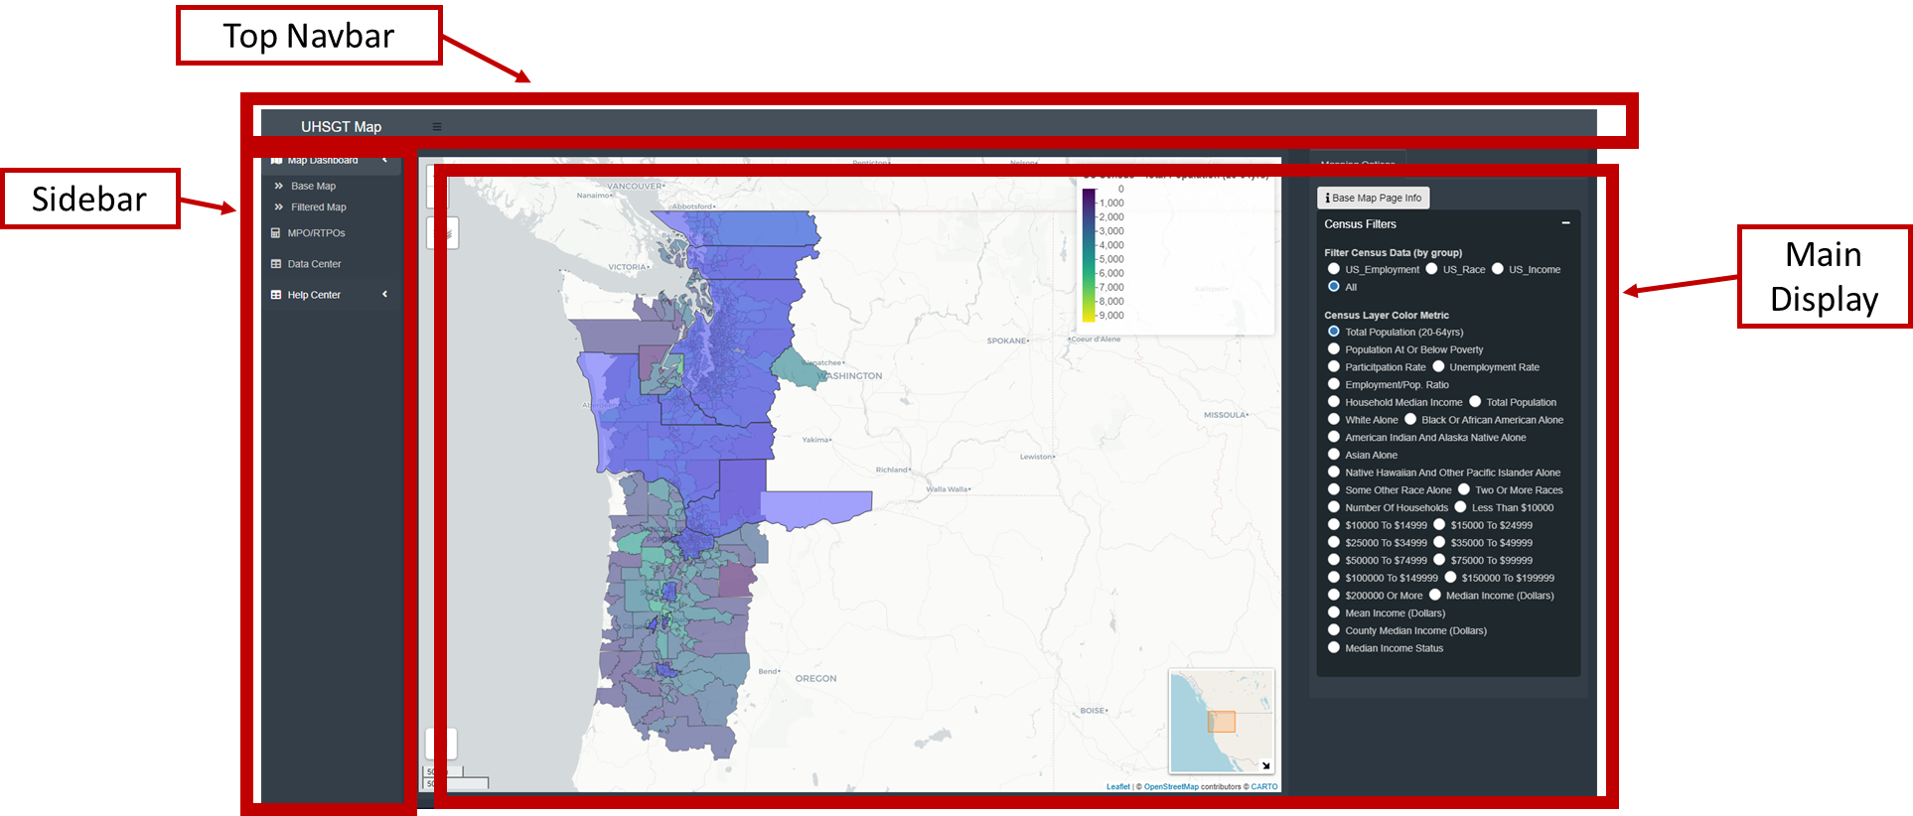
\includegraphics{./www/dashboard_overview.png}

Top Header Bar

\begin{itemize}
\tightlist
\item
  This bar is intentionally bare
\item
  It contains the title of the dashboard and a menu-icon (three stacked
  bars)
\item
  Clicking on the menu-icon will collapse the left sidebars - resulting
  in a wider main display
\end{itemize}

Left Sidebar

\begin{itemize}
\tightlist
\item
  As mentioned above, the sidebar can be collapsed to make more room for
  the main display

  \begin{itemize}
  \tightlist
  \item
    The sidebar can still be used to navigate the site when collapsed
  \end{itemize}
\item
  The left sidebar contains the links to different pages on the
  dashboard

  \begin{itemize}
  \tightlist
  \item
    \textbf{Map Dashboard} is the default page and contains two
    sub-pages

    \begin{itemize}
    \tightlist
    \item
      The \textbf{Base Map} page displays the base map and map input
      controls on the right sidebar
    \item
      The \textbf{Filtered Map} page contains all of the features that
      allow for user-defined geometry, map sub-setting, and metric
      aggregation
    \end{itemize}
  \item
    The \textbf{Regional Planning} page contains information pertaining
    to US MPOs and Canadian Regional Districts (RTDs)

    \begin{itemize}
    \tightlist
    \item
      In particular, this page details when specific planning documents
      will be redrafted and published by the MPOs/RTDs
    \item
      The US documents tracked by this dashboard are the Comprehensive
      Economic Development Strategy (CEDS), Regional Transportation Plan
      (RTP), and the Transportation Improvement Program (TIP)
    \item
      The Canadian documents traced by this dashboard are equivalent to
      that of those specified above
    \end{itemize}
  \item
    The \textbf{Data Center} page contains tables detailing the layers
    used for the base map
  \item
    The \textbf{Help Center} widget does not link to a new page but
    displayed additional help and information buttons when clicked
  \end{itemize}
\end{itemize}

Main Display

\begin{itemize}
\tightlist
\item
  All clickable page links (except ``Help Center'') on the left sidebar
  will take the user to new display page
\item
  The main displays are made of containers that hold/show maps, plots,
  buttons, or inputs that the user can interact with
\end{itemize}

\hypertarget{dashboard-pages}{%
\subsection{Dashboard Pages}\label{dashboard-pages}}

This section describes the different pages of the dashboard and their
functionality in more detail.

\hypertarget{base-map}{%
\subsubsection{Base Map}\label{base-map}}

This page displays the base corridor map and it's census inputs.

The default map displays a multitude of layers depicting jurisdictional
boundaries and important transportation features located along corridor.
The extent of the base map reaches from Eugene, Oregon to Vancouver,
British Columbia and from the Pacific Ocean to the Cascades. Many of the
map layers' extents were much larger than what is currently shown in the
dashboard but were buffered/reduced to limit computational load and to
narrow the region for planning efforts. As implied earlier, the map
contains layers for British Columbia, Washington, and Oregon - not all
states or regions have the same type of data or types of layers
available to them. This was a result of data being available for certain
regions and not others as well as differences in data between the US and
CA.

\hypertarget{map-info}{%
\paragraph{Map Info}\label{map-info}}

\begin{itemize}
\tightlist
\item
  The map is interactive

  \begin{itemize}
  \tightlist
  \item
    It can be manipulated using your cursor
  \item
    Perform zoom and pan operations by clicking on the map and rolling
    the mouse wheel or drag the map, respectively
  \end{itemize}
\item
  Layers can be hidden or displayed by clicking on layers contained in
  the map layer icon

  \begin{itemize}
  \tightlist
  \item
    See the upper left-hand corner of the map
  \item
    The default displayed layers are Regional Planning and US/CA Census
    tracts
  \item
    The US and CA Census layer's name will change depending on what
    Census metric is being used to color scale census tracts
  \item
    The default metric for the US/CA Census layers are Total Population
    and Population(2016), respectively

    \begin{itemize}
    \tightlist
    \item
      The metric used to color US Census tract polygons can be changed
      by interacting with the Census Filters menu

      \begin{itemize}
      \tightlist
      \item
        See the sidebar drop-down to the right of the main display
      \end{itemize}
    \end{itemize}
  \end{itemize}
\item
  The number of metrics per US an CA can be reduced

  \begin{itemize}
  \tightlist
  \item
    Filter Census Data (by group) changes/limits the available Census
    Layer Color Metric options and which metrics are displayed on the
    map
  \end{itemize}
\item
  The right sidebar contains inputs the user can use to augment the map

  \begin{itemize}
  \tightlist
  \item
    The user can limit the number of Census metrics shown in the map
    pop-up window by
  \item
    The user can change the census layer coloring be changed by
    interacting with the Census Filters menu
  \item
    The colors used for the US and CA census layers can be changed
    individually
  \item
    The metric used to color the map will also be displayed in the
    histogram below each menu input
  \end{itemize}
\item
  The right sidebar displays two plots for the US and Canadian drop
  downs

  \begin{itemize}
  \tightlist
  \item
    These plots display histograms for the selected variable used to
    color each census layer by
  \item
    The top plot displays the histogram for the entire corridor for the
    specified hairball
  \item
    The bottom plot displays the histogram for a subset of the corridor
    for the specified variable

    \begin{itemize}
    \tightlist
    \item
      This subset is determined by the map bounding box created by the
      map viewer pane
    \item
      Example: if the user zooms into the map, they will make this
      bounding box smaller this displaying a smaller number of census
      tracts, the subset map will redraw the histogram only using the
      census tracts seen in the viewer pane/bounding box
    \end{itemize}
  \end{itemize}
\end{itemize}

\hypertarget{filtered-map}{%
\subsubsection{Filtered Map}\label{filtered-map}}

This page enables the user to define new geometries to use to spatially
filter the default corridor map. The subset returns all layers and
features that it overlaps with and removes all layers that it has no
interaction with. Metrics for the remaining census tracts are aggregated
and returned to the user both visually in a series of plots and in
tabular form. The subset aggregates can be compared to the corridor
level aggregates to investigate how user defined spatial subset deviates
from the corridor as a whole. For example, a user might be interested in
equity and a specific demographic's representation for a potential
Right-of-Way (ROW). The user draws a line on the map representing the
proposed ROW, all relevant layer and map features are returned to the
user once they initiate the subset process. They can then investigate
their question regarding equity with respect to the proposed ROW. The
user-defined features and resulting aggregated data can be downloaded -
these processes are described below. The data created via the subset are
available for both US and CA layers.

This page is composed of two containers - the top input container and
the lower tab box. The top input container houses buttons and inputs
that the user can use to define and initiate the map sub-setting and
metric aggregation process. The tab box contains a number of tabs that
house the sub-setting features and the resulting maps, plots, and
tables.

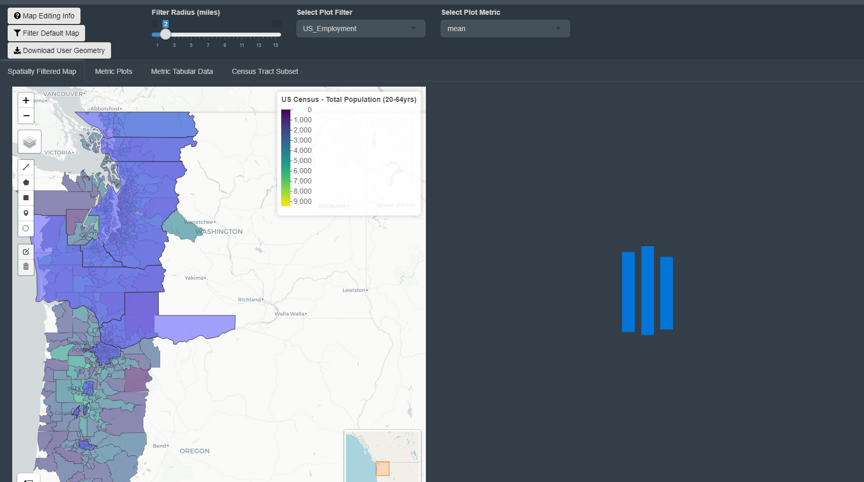
\includegraphics{./www/map_edit.png}

\hypertarget{page-description}{%
\paragraph{Page Description}\label{page-description}}

\begin{itemize}
\tightlist
\item
  Top Input Container

  \begin{itemize}
  \tightlist
  \item
    Contains the buttons used to filter map and download shapefile
  \item
    Displays the inputs to change the buffer applied to the user's
    geometry and selector for variables to show the box plots
  \end{itemize}
\item
  Spatially Filtered Maps

  \begin{itemize}
  \tightlist
  \item
    This is the default tab for the tab box
  \item
    This tab Displays two maps - the left is editable and the right
    displays those edits and returns buffered corridor map

    \begin{itemize}
    \tightlist
    \item
      The buffered map (right map) will not load until the process has
      been initiated by the user
    \end{itemize}
  \end{itemize}
\item
  Metric Plots

  \begin{itemize}
  \tightlist
  \item
    This tab displays plotted aggregated metrics based on the geometries
    defined by the user geometries and the resulting subsetted corridor
  \item
    The top plot displays the Percent Difference between the corridor
    and corridor subset for all US Census variables

    \begin{itemize}
    \tightlist
    \item
      The user can choose which metric is displayed resulting from the
      aggregation process

      \begin{itemize}
      \tightlist
      \item
        The median, mean, min, max, or standard deviation of the
        aggregated metrics - mean is the default implying the values are
        the average of the metrics for the subset census tracts and the
        corridor census tracts
      \end{itemize}
    \item
      E.g.
      100*(mean(Subset\_Metric)-mean(Corridor\_Metric))/mean(Corridor\_Metric)
    \item
      Green indicates that the subset aggregate is larger than the
      corridor level aggregate (does not imply ``being better'' than)
    \item
      Both of these plots are interactive

      \begin{itemize}
      \tightlist
      \item
        The user can hover-over features with the tool-tip to display
        more information
      \item
        The user can zoom in on plot features using the zoom controls
      \item
        The user can take pictures of the plots and save them using the
        camera feature
      \end{itemize}
    \end{itemize}
  \item
    The bottom plot displays the same data but in box-plot form

    \begin{itemize}
    \tightlist
    \item
      The box plots indicate the central tendency and spread of the US
      Census metrics over the corridor and subsetted census tracts
    \item
      The user defines which variables to include in the plot by
      clicking on variables in the table left-adjacent
    \item
      Like above, this plot is also fully interactive
    \end{itemize}
  \end{itemize}
\item
  Metric Tabular Data

  \begin{itemize}
  \tightlist
  \item
    This tab displays the same information as the above plots do but in
    tabular form
  \item
    The data in this table can be downloaded using the buttons located
    on the top of the table
  \end{itemize}
\item
  Census Tract Subset

  \begin{itemize}
  \tightlist
  \item
    This tab contains a table detailing which census tracts were
    selected by the subset
  \item
    The data in this table can also be downloaded and should be
    downloaded along with the tabular metrics above
  \end{itemize}
\end{itemize}

\hypertarget{subset-process-description}{%
\paragraph{Subset Process
Description}\label{subset-process-description}}

\begin{itemize}
\tightlist
\item
  The user defines a new geometry - polygons, lines, points, etc - using
  the left toolbar on the left hand map (see Spatially Filtered Maps
  tab)
\item
  The user defines a buffer (default 1 mile) to be applied to their
  geometry (see top Navbar)
\item
  The user submits their selections and initiates the filtering and
  aggregation process by clicking the Filter Default Map button (see
  Navbar above)
\item
  The user defined features and the resulting subset will be displayed
  on the right hand map (see)
\item
  US Census metrics (corridor and subsets) are displayed on the Subset
  Plots and Subset Data tabs
\item
  The user has the option to download their geometry by pressing the
  Download User Geometry button (see Navbar above)
\end{itemize}

\hypertarget{regional-planning-page}{%
\subsubsection{Regional Planning Page}\label{regional-planning-page}}

This page contains information about the regional agencies responsible
for transposition planning along the corridor. In the US, regional
transportation planning is performed by metropolitan planning
organizations (MPO) or regional transportation planning organizations
(RTPO) - these organizations are federally mandated and federally funded
and are in place to ensure regional cooperation with regards to
transportation planning. In Canada, the regional planning is performed
at the Regional District level - the map currently only contains
regional planning documents for Vancouver Metro/TransLink. This layer of
governance directs and allocates investments for transportation
projects, establish shared vision and goals for the future of the
regions, and acts as a conduit that facilitate collaboration between
residents, interested parties, and other levels of government both at
the federal, state, and local levels. In acting in the capacity stated
above, regional transportation planners produce a number of publications
which detail both short-range project funding and long-range
transportation planning. For the US regional planners, these documents
are the Transportation Improvement Program (TIP) and the Regional
Transportation Plan (RTP), respectively. The Canadian regional
transportation planners also release documents that are similar to and
act in the same capacity as the documents stated above - they are
currently classified in the dashboard with the TIP, RTP, or CEDS
acronyms for simplicity.

This page contains a few features to help track these documents and to
provide information on the US and CA regional planning organizations:

Census Metrics Table

\begin{itemize}
\tightlist
\item
  This table is the result of spatially aggregating the census tract
  layers using the US MPO/RTPO boundaries

  \begin{itemize}
  \tightlist
  \item
    This table does not currently contain data for Vancouver Metro
  \end{itemize}
\end{itemize}

Documents Timeline

\begin{itemize}
\tightlist
\item
  This plot graphically depicts when the different US/CA regional
  planning organization's planning documents are expected to be
  rewritten or updated

  \begin{itemize}
  \tightlist
  \item
    The RTP documents are supposed to be updated every four years
  \item
    The TIP documents are supposed to be updated every year
  \item
    The expected document update dates seen in this plot are estimates
  \item
    These estimates are based off of the information above and when the
    document was published or last updated
  \item
    IT was to determine for some of the documents when they were last
    updated and some of the information contained in this plot may be
    incorrect
  \end{itemize}
\end{itemize}

\hypertarget{data-center}{%
\subsubsection{Data Center}\label{data-center}}

This page allows the user to examine and retrieve the data contained in
the base map. This page contains two tables - the left hand table
contains information on all the layers which are currently included in
the base map and the right hand table details the information contained
in each layer. All layers have been previously processed in order to
remove superfluous information, clean or reconstruct data of poor
quality, spatially buffer to limit the original extent of the data, or
two combine similar data that were retreived from separate sources.
Links are provided to the data's original source as well as features
that allow the user to download the processed data.

Default Map Data Layers table

\begin{itemize}
\tightlist
\item
  Contains information for all layers in base map
\item
  Contains notes on the data layer - enabled by user click
\item
  Contains links to the original data source - enabled by user click
\item
  Clicking on a singular data layer will select that layer to be
  displayed in the right-hand table
\item
  The contents of this table can be downloaded or copied by using the
  buttons at the top of the table
\end{itemize}

Raw Data for Selected Layer

\begin{itemize}
\tightlist
\item
  Displays the data for the layer selected via user row selection of the
  left hand table
\item
  Displays all the information for selected layer that is shown in the
  base map
\item
  The contents of this table can be downloaded or copied by using the
  buttons at the top of the table
\end{itemize}

\hypertarget{help-center}{%
\subsubsection{Help Center}\label{help-center}}

Selecting this menu item will not generate a new display window but will
two buttons directly below in the sidebar menu. These buttons re-display
the into-modal seen when the page first loads and takes you to this
document.

\hypertarget{sharing-this-dashboard}{%
\subsection{Sharing this Dashboard}\label{sharing-this-dashboard}}

This dashboard's main intent is to enable UHSGT planners to identify
corridor stakeholders early in the planning process. This dashboard was
not meant to be a public facing product or made for the use by the
general public. Users who have been granted access to this dashboard
should ask for permission before sharing this with others. Please
contact your WSDOT representative for permission to do so.

\end{document}
